\PassOptionsToPackage{backref=page}{hyperref}
% %%% === ADDITIONAL PACKAGES
% \usepackage{animate}
\usepackage{caption}
\usepackage{subcaption}
\usepackage{tikz}
\usepackage{cancel}
\usepackage{booktabs}
\usepackage{stmaryrd}
\usepackage[export]{adjustbox}
\usepackage{fontawesome5}
\usepackage{algorithmic}
\usepackage{amsmath, amssymb}
\usepackage{yfonts}
\graphicspath{{./}}

% % \LinesNumbered
\newcommand{\theHalgorithm}{\arabic{algorithm}}
% \newcommand{\theHtable}{\thetable}
\usepackage[ruled,vlined]{algorithm2e}
\renewcommand{\algorithmicrequire}{\textbf{Input:}}
\renewcommand{\algorithmicensure}{\textbf{Output:}}
\newcommand{\vect}[1]{\boldsymbol{\mathbf{#1}}}

% %%% === CONDITIONAL PACKAGE
\usepackage{ifthen}

%%% === TEMPLATE
\usepackage{fontspec}
\usepackage{polyglossia}

% Set the main language to Russian
% \setmainlanguage{russian}

% Set Computer Modern Unicode (CMU) as the main font for both Latin and Cyrillic
\newfontfamily\cyrillicfont{CMU Serif}
\newfontfamily\cyrillicfontsf{CMU Sans Serif}
\newfontfamily\cyrillicfonttt{CMU Typewriter Text}

\setmainfont{CMU Serif}          % For regular (serif) text
\setsansfont{CMU Sans Serif}      % For sans-serif text
\setmonofont{CMU Typewriter Text} % For monospaced (typewriter-style) text
\DeclareSymbolFontAlphabet{\mathbb}{AMSb}
\setmathfont{CMU Sans Serif}

\setbeamerfont{title}{series=\bfseries}
\setbeamerfont{frametitle}{series=\bfseries, size=\fontsize{12}{14}}
\setbeamerfont{normal text}{series=\mdseries}

\setbeamersize
{
    text margin left=0.214cm,
    text margin right=0.214cm
}

% \usefonttheme[onlymath]{serif}
\setbeamertemplate{bibliography item}{\insertbiblabel}
\setbeamertemplate{itemize items}[circle] % For level-1 itemize
\setbeamertemplate{itemize subitem}[circle] % For level-2 (subitems)
\setbeamertemplate{itemize subsubitem}[circle] % For level-3 (subsubitems)
\captionsetup[figure]{name=Рис.}

% Футер: логотип слева, название лекции по центру, телеграм и номер страницы справа
\setbeamertemplate{footline}{
  \leavevmode%
  \begin{beamercolorbox}[wd=\paperwidth,ht=3.2ex,dp=1.4ex,leftskip=0.5cm,rightskip=0.5cm]{structure}
    \begin{minipage}[c]{0.25\paperwidth}
      \raggedright
      \href{https://sleep3r.ru/presentations/t-ai}{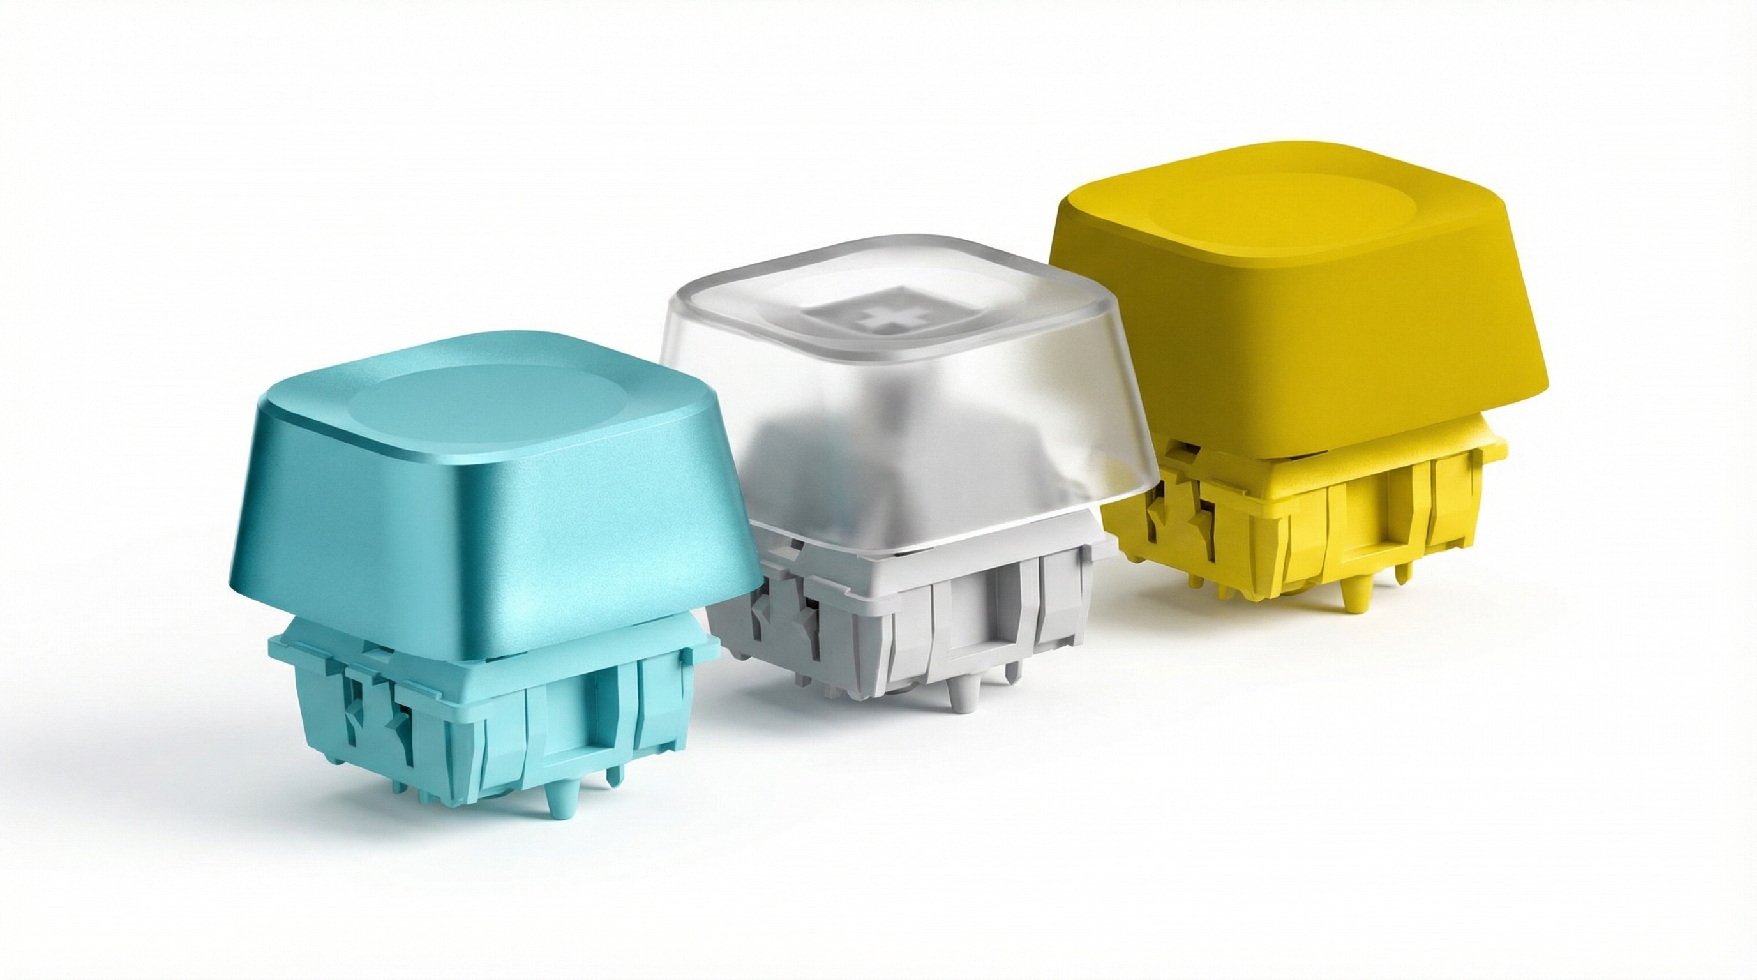
\includegraphics[height=0.32cm]{logo.pdf}}
    \end{minipage}%
    \begin{minipage}[c]{0.45\paperwidth}
      \centering
      {\tiny\insertshorttitle}
    \end{minipage}%
    \begin{minipage}[c]{0.25\paperwidth}
      \raggedleft
      \usebeamerfont{footline}%
      \href{https://t.me/sleep3r}{\faTelegram}
      \hspace{0.4cm}
      \insertframenumber{} / \inserttotalframenumber
    \end{minipage}%
  \end{beamercolorbox}
  \vskip0pt%
}

\setbeamerfont{footline}{size=\small}

\usenavigationsymbolstemplate{}

% %%% === ADDITIONAL COMMANDS
\newcommand*{\Scale}[2][4]{\scalebox{#1}{$#2$}}%
\newcommand{\argmin}{\operatornamewithlimits{argmin}}
\newcommand{\argmax}{\operatornamewithlimits{argmax}}
\newcommand{\la}{\langle}
\newcommand{\ra}{\rangle}

%%% === BACKGROUND IMAGE SETUP
\AtBeginDocument{
  \ifthenelse{\isundefined{\bgimage}}{
    % No background image specified
  }{
    \setbeamertemplate{title page}{
      \begin{tikzpicture}[remember picture,overlay]
        \node[anchor=center, xshift=0pt, yshift=0pt] at (current page.center) {
          \includegraphics[width=1.05\paperwidth, height=1.05\paperheight]{\bgimage}
        };
        \node[fill=white, fill opacity=0.7, text opacity=1, inner sep=10pt, rounded corners=10pt] at (current page.center) {
          \begin{minipage}{0.5\paperwidth}
            \centering
            \usebeamerfont{title}\inserttitle\par
            \vspace*{0.5cm}
            \usebeamerfont{author}\insertauthor\par
            \vspace*{0.5cm}
            \usebeamerfont{institute}\insertinstitute\par
          \end{minipage}
        };
      \end{tikzpicture}
    }
  }
}